\documentclass[11pt]{article}
\usepackage{amsmath, amssymb, amscd, amsthm, amsfonts}
\usepackage{graphicx}
\usepackage{subcaption}

\graphicspath{ {./Images/} }
\usepackage{hyperref}

\oddsidemargin 0pt
\evensidemargin 0pt
\marginparwidth 40pt
\marginparsep 10pt
\topmargin -20pt
\headsep 10pt
\textheight 8.7in
\textwidth 6.65in
\linespread{1.2}

\title{Trust Region Policy Optimization - Implementation}
\author{Pietro Nardelli \\ \\
        Master's Degree in Artificial Intelligence and Robotics \\
        Department of Computer, Control and Management Engineering \\
        Sapienza University of Rome}

\date{January 2020}

\begin{document}

\maketitle

\section{Introduction}
Trust Region Policy Optimization is an algorithm that make several
approximations to a theoretical iterative procedure for optimizing policies with
guaranteeed monotonic improvement. Despite its approximations that deviate from
the theory, TRPO tends to give monotonic improvement, while little tuning of
hyperparameters. This algorithm is effective for optimizing large nonlinear
policies such as neural networks. The algorithm has been tested on two different
openAI gym environments. Gym library is a collection of test problems that can
be used to test reinforcement learning algorithms.

\section{Environments}

\subsection{MountainCarContinuous-v0}
An underpowered car must climb a one-dimensional hill to reach a target. The
action (engine force applied) is allowed to be a continuous value.
The target is on top of a hill on the right-hand side of the car. If the car reaches it or goes beyond, the episode terminates.
\\
On the left-hand side, there is another hill. Climbing this hill can be used to
gain potential energy and accelerate towards the target. On top of this second
hill, the car cannot go further than a position equal to -1, as if there was a
wall. Hitting this limit does not generate a penalty.
\\
The observations are CarPosition and CarVelocity and the only action permits to
push the car on the left (negative values) or on the right (negative values).
\\
Reward is 100 for reaching the target of the hill on the right hand side,
minus the squared sum of actions from start to goal.

This reward function raises an \textbf{exploration challenge}, because if the agent does
not reach the target soon enough, it will figure out that it is better not to move,
and won't find the target anymore.
\\
To consider the problem solved, the reward should be over 90.


\subsection{LunarLanderContinuous-v0}
A lunar lander is a spacecraft designed to land on the Moon. Landing pad is always at coordinates
(0,0). Reward for moving from the top of the screen to landing pad and zero speed is about 100-140
points. If lander moves away from landing pad it loses reward back. Episode finishes if the lander
crashes or comes to rest, receiving additional -100 or +100 points. Each leg ground contact is +10.
Firing main engine is -0.3 points each frame (fuel is infinite). Solved is 200 points. Action is two
real values vector from -1 to +1. First controls main engine, [-1,0] off, [0,1] throttle from 50\%
to 100\% power, Second value [-1.0,-0.5] fire left engine, [0.5,1.0] fire right engine, [0.5,0.5]
off.
\begin{figure}[h!]
        \centering
        \begin{subfigure}[b]{0.4\linewidth}
                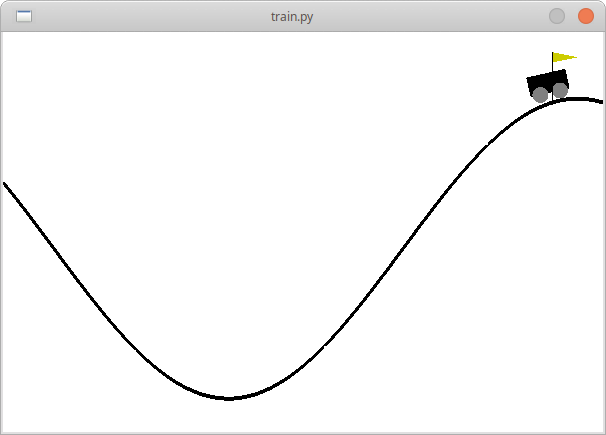
\includegraphics[width=\linewidth]{mountain_screen}
                \caption{}
        \end{subfigure}
        \begin{subfigure}[b]{0.4\linewidth}
                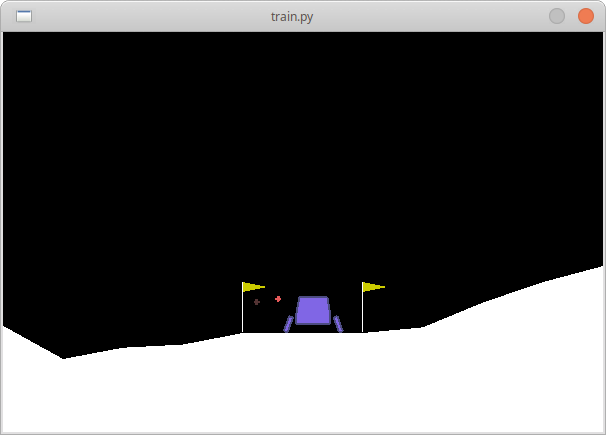
\includegraphics[width=\linewidth]{lunar_screen}
                \caption{}
        \end{subfigure}

        \caption{ Both the environments just described. (a) MountainCarContinuous-v0 when reaching the goal position.(b) LunarLanderContinuous-v2 when reaching the landing pad.}
        \label{fig:screens}
\end{figure}

\section{TRPO algorithm}\label{section-trpo}
Let $\pi$ denote a stochastic policy and let $\eta(\pi)$ denote its expected discounted reward. The
advantage function $A_{\pi} = Q_{\pi}(s, a) - V_{\pi}(s)$ is the difference between state-action
value function and value function. We can prove that any policy update $\pi \rightarrow \tilde{\pi}$
that has a nonnegative expected advantage at every states is guaranteeed to increase the policy
performance $\eta$, or leave it constant in the case that the expected advantage is zero everywhere.
Intuitively, we can think of it as measuring how good the new policy is with regard to the average
performance of the old policy. However, in the approximate setting, it will typically be
unavoidable, due to estimation and approximation error, that there will be some state s for which
the expected advantage is negative. This is the idea at the base of the policy iteration algorithm
that is a type of minorization-maximization algorithm. The evolution of this kind of algorithm is
called Trust Region Policy Optimization (TRPO), which uses a constraint on the Kullback–Leibler (KL)
divergence rather than a penalty to robustly allow large updates. The KL divergence is a measure of
how one probability distribution $P$ is different from a second probability distribution $Q$ that is
a reference for the first one: $D_{KL}(P||Q)$.

\begin{figure}[t]
        
\includegraphics[width=15cm]{functions}
        \centering
        \caption{In practice, if penalty coefficient is included in the objective function,
        the step size will be very small, leading to long training time.
        Consequently, a constraint on the KL divergence is used to allow a larger step size
        while guarantee robust performance.}
        \label{fig:functions}
\end{figure}

In fact, supposing that we used the penalty coefficient C recommended by theory, the step sizes
would be very small (fig. \ref{fig:functions}). One way to take larger steps in a robust way is to use a constraint
on the KL divergence between new policy and old policy (trust region constraint):
\begin{equation}
        \begin{split}
        maximize_{\theta} \ L_{\theta_{old}}(\theta)
        \\ \label{eq:1}
        subject \  to \ D_{KL_{max}}(\theta_{old}, \theta) \leq \delta
        \end{split}
\end{equation}

Since eta is hard to optimized, $L$ is a local approximation to $\eta$. Another
assumption is that $D_{KL}(\theta|| \tilde{\theta}) :=
D_{KL}(\pi_{\theta}||\pi_{\tilde{\theta}})$. This problem imposes a constrain that the KL
divergence is bounded at every point in the state space. While it's motivated by the
theory, this problem is impractical to solve due to large number of constraints.
Unfortunately, it is not solvable as there are a infinitely large number of
states: we can used a heuristic approximation which considers the avarage KL
divergence $\bar{D_{KL}}$. Our optimization problem in equation (\ref{eq:1}) is exactly
equivalent to the following one (written in terms of expectations, replacing some terms):

\begin{equation}
        \begin{split}
        maximize_{\theta} \ E_t[\frac{\pi_{\theta}(a_t, s_t)}{\pi_{\theta_{old}}(a_t, s_t)}A_t]
        \\ \label{eq:2}
        subject \  to \ D_{KL_{max}}(\theta_{old}, \theta) \leq \delta
        \end{split}
\end{equation}

The objective function is also called a “surrogate” objective function as it contains a
probability ratio between current policy and the next policy. The subset of region lies
within the constraint is called trust region. As long as the policy change is reasonably
small, the approximation is not much different from the true objective function By
choosing the new policy parameters which maximizes the expectation subject to the KL
divergence constraint, a lower bound of the expected long-term reward $\eta$ is guaranteed.
\\
In the trust region, we limit our search within a region controlled by $\delta$.
Mathematically, we can prove that such region guarantees that its optimal policy will
outperform the current one until it reaches a local or global optimal.
\\
A practical algorithm could be:

\begin{enumerate}
        \item Use a procedure to collect a set of state-action pairs.
        \item By averaging over samples, construct the estimated objective and constraint
        in equation \ref{eq:2}.
        \item Approximately solve this contrained optimization problem to update the
        policy's parameter vector $\theta$.

\end{enumerate}
The third point has been done by the author with a conjugate gradient algorithm followed
by a line search, or in other words, compute a search direction and perform a line search
in that direction.
The search direction is computed by approximately solve the equation $Ax = g$ where $A$ is
the Fisher information matrix (part of the KL divergence). Given that this matrix is
costly in large-scale problems, the conjugate gradient allows us to approximately solve
this equation without forming the matrix itself.
Having computed the search direction, it's necessary to compute the maximal step lenght
such that the constraint is satisfied.
Then, the line search has been used to ensure improvement of the surrogate objective and
satisfaction of the KL divergence constraint.
\\
As far as the author specifies that this is an efficient method to solve the problem, it's
really hard to implement practically. Given this difficulties in the implementation, I've
decided to solve the constraint optimization problem (eq. \ref{eq:2}), using an
handcrafted solution which uses gradient descent, even if it is not the most efficient
solution (fig. \ref{fig:gradient}), as we will see in the next section.


\section{Implementation}


\begin{figure}[t]
        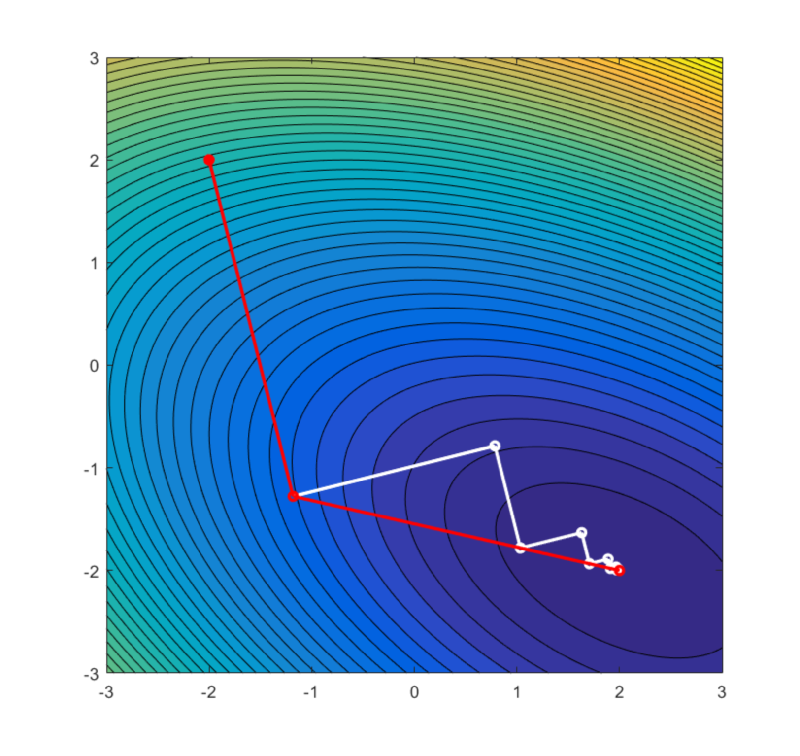
\includegraphics[width=9cm]{gradient}
        \centering
        \caption{Difference between conjugate gradient (red line) and gradient descent
        (white line). As we can see che conjugate gradient can reach the minimum point of
        the function in less steps.}
        \label{fig:gradient}
\end{figure}



It has been used the single-path method in which a set of trajectories is generated via
simulation of the policy from $s_0$ for some number of timesteps.

\begin{figure}[t]
        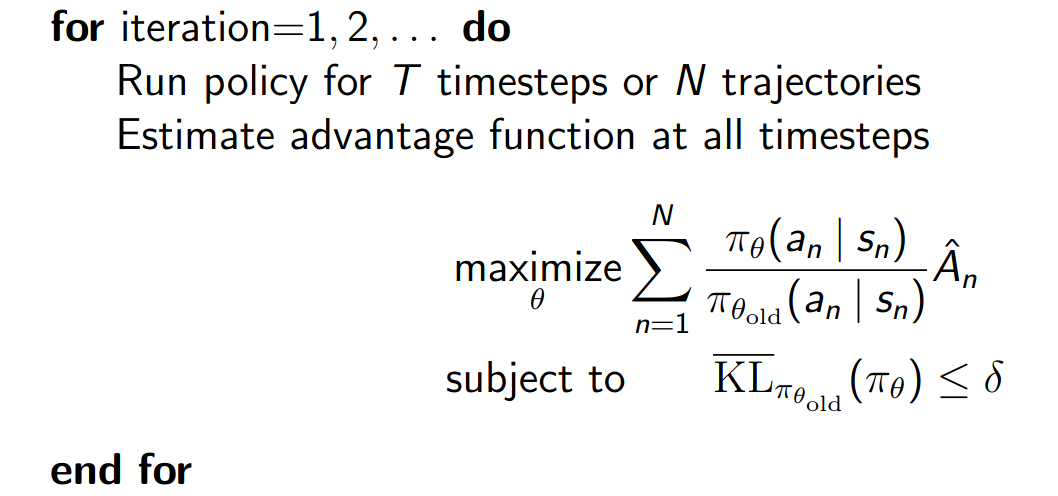
\includegraphics[width=9cm]{pseudocode}
        \centering
        \caption{Pseudocode for TRPO algorithm.}
        \label{fig:pseudocode}
\end{figure}

The value function is approximated through a neural network. This value function
approximation has to be done so we can calculate the advantage. The value function NN has
been fitted with X equals to observations and Y equals to discounted sum rewards (so we
can minimize the difference between pedicted vs true value with a MSE). The disc sum
rewards has been calculated from every state to the last one of each trajectory. The advantage is
needed to calculate the loss function for the Policy NN and to train the NN itself. The
policy NN has the aim to return also the sample of the next action to take from a
particular observation. Policy NN has been trained with a multi input for tot epochs and
the train would go until KDL < delta. In that case, the NN backtrack to a previous setting
(weights loading) so the contraint has been respected (substituing the line search from
the original paper). Altough theorically the constraint is respected, given the
approximation of the value function it's not possible to obtain a positive advantage
everytime. For this reason, as we will se in the plots in the next paragraph, the policy
will have monotonic improvement only in the general picture (some descreases could
happen). The conjugate gradient algorithm even if more efficient has not been used because
it wasn't possible to implement in a simple way. For this reason instead of it a gradient
ascent on the loss policy has been used (adam). So at the end of each episode batch
there's this policy update and value function fit so our neural networks are everytime
updated. The total train set (collection of all the trajectories) has been updated too.
The batch size is really low to do not saturate the RAM of my computer.

The input of the POLICYNN is observation and the output are means and logvars.
When we compute the loss we will return also the KL divergency (it's not the real output
of the NN).

Each update should use "predict" so we can compute the KL (and the loss, in particular).
The update is made over tot epochs and when KL diverges from delta, stop and backtrack to
the previous state of the neural network.

\begin{itemize}
        \item Discount factor $\gamma$:
        \item D-KL target value $\delta$
        \item Batch size $bs$
        \item Hidden layer 1 size $h1s$
        \item Epsilon-greedy $\epsilon$
        \item Initial log variance $iLogVar$
        \item Policy learning rate $Plr$
        \item Policy epochs $PVe$
        \item Function value learning rate $FVlr$
        \item Function value epochs $FVe$
        \item 
\end{itemize}



\section{Results}
The results has been obtained training the agent for a sufficient quantity of episodes.
Before taking the right results, various tests have been made changing the parameters of
the algorithm.


       
We should choose delta and alpha carefully to permits to the algorithm to avoid steps too
large and decide what e > 10 circa. mountain car:
$$500 episodes reach the solution (90 score). Env_seed (11), lr 0.0003$$

\begin{figure}[h!]
        \centering
        \begin{subfigure}[b]{0.6\linewidth}
                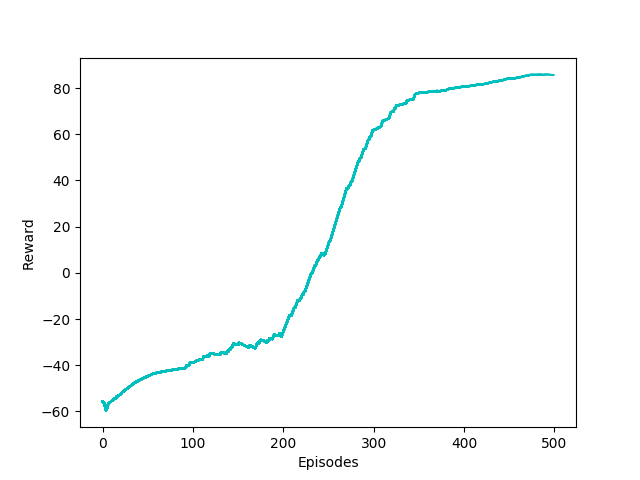
\includegraphics[width=\linewidth]{mountain_plot}
                \caption{}
        \end{subfigure}
        \begin{subfigure}[b]{0.6\linewidth}
                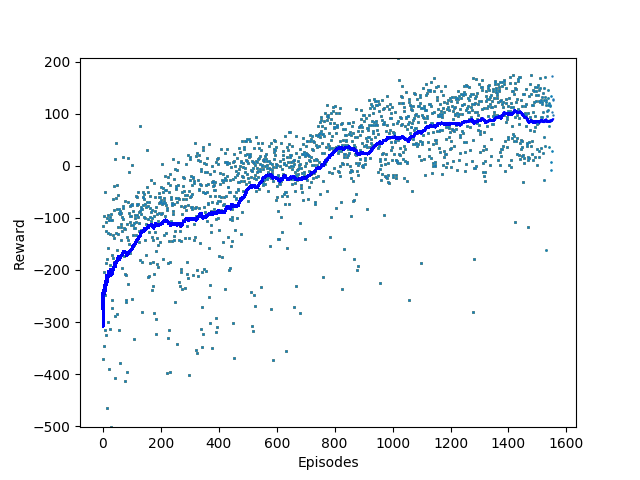
\includegraphics[width=\linewidth]{lunar_plot}
                \caption{}
        \end{subfigure}

        \caption{ Plot of the rewards obtained for each epoch by the agent. The environments in which the agent operates are (a) MountainCarContinuous-v0 and (b) LunarLanderContinuous-v2.}
        \label{fig:plots}
\end{figure}

\end{document}
